\subsection{Ether}
Ether~\cite{ether} is a malware analysis platform that utilizes 
Intel VT's hardware virtualization extensions, and theoretically it has no presence 
in the guest operating system. It uses native CPU instructions, thus does not suffer from 
incomplete or inaccurate system emulation such as hardware emulators do. 
Ether also comes with a rich feature set, thus it can monitor 
all the memory write attempts of the guest, trace the instructions and 
system calls of in-guest processes, and unpack a wide range of protected binaries. 
As a result, malware cannot detect the presence of Ether. In that paper, 
they evaluated Ether and several other state-of-the-art analyzers on the obfuscation techniques 
used to obfuscate 25,000 recent malware samples. The results show that Ether remains transparent 
and defeats the obfuscation tools that evade the existing approaches. 
Ether's system architecture is represented in Figure~\ref{fig:ether} below.

\begin{figure}[!h]
	\centering
	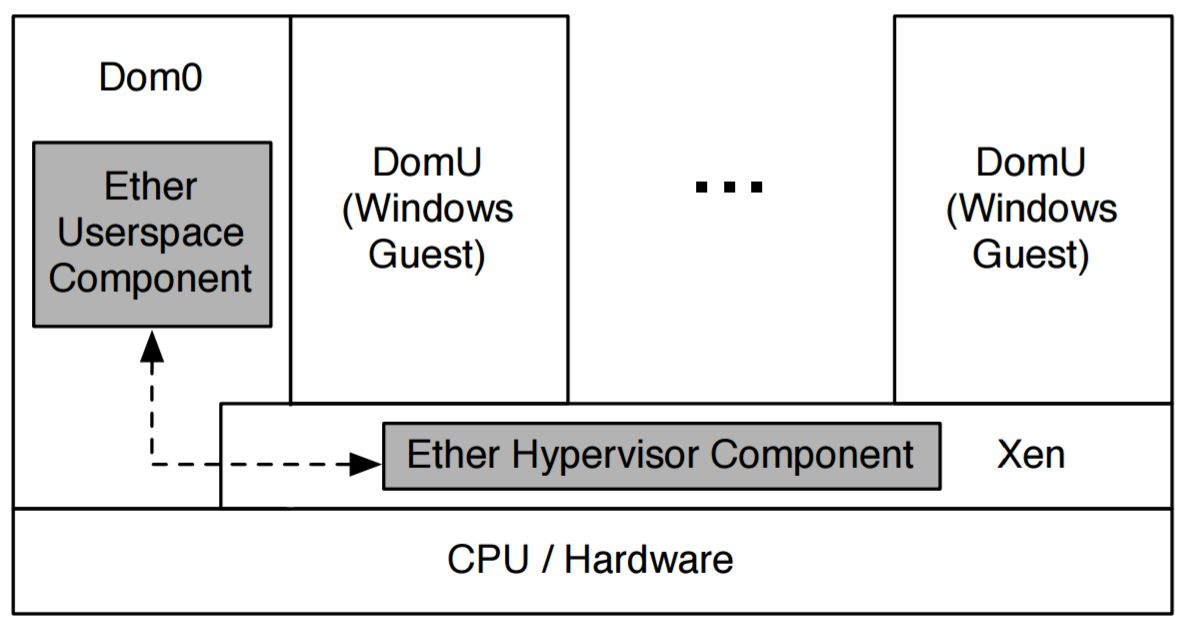
\includegraphics[width=\linewidth]{figure/ether.png}
	\caption{Ether's system architecture.}
	\label{fig:ether}
\end{figure}

\subsection{nEther}
P{\'e}k \textit{et al.} introduced novel approaches that make the detection of 
hardware assisted virtualization platforms and out-of-the-guest 
malware analysis frameworks possible~\cite{nether}. In order to demonstrate their concepts, 
they implemented a scalable and flexible application framework over Window XP 
called \textit{nEther} which can practically disclose the presence of both 
\textit{Ether}~\cite{ether}, and Intel VT by executing multiple feature tests. 
The system overview of nEther is depicted in Figure~\ref{fig:nether} and 
their proposed feature tests consist of three parts as follows: 1) timing information, 
2) CPUID information, and 3) CPU Errata. 

The use of timing information is a well-known techinique to detect the presence 
of traditional debuggers. The simplest way to get timing information is 
the use of internal timers and periodic interrupt sources such as the Time-Stamp Counter(TSC), 
Periodic Interrupt Timper (PIT), and so on. In case of out-of-the-guest malware analyser, 
it falsify internal timers in order to fool a timing test and provide transparency. 
However, the correct manipulation of timing cannot be guaranteed in all the circumstances. 
As a result, nEther can detect the existence of Ether, based on a contradiction 
raised by clock cycle manipulation where the analyzer returns an adjusted cycle 
difference to hide its presence.

The CPUID instruction returns processor identification and feature information 
depending on the content of general registers EAX and ECX. These could be exploited 
by anlyzer detectors as various modifications of the system can be retrieved. 
In case of Ether, it does alter a few bits of information that could be returned 
by the correct configuration of CPUID. Therefore, nEther can detect Ether 
by checking a few bits returned by a CPUID that are specific to Ether.

CPU Errata refer to the collection of design defects or errors and 
it strongly depends on CPU models. nEther exploits bugs in the Core 2 Duo family, 
called AH4 Erratum which unintendedly updates the Last Exception Recored(LER) MSR. 
This errata is not implemented in hardware-assisted-virtualization solutions, such as Xen. 
In other words, this bug will not happen in the hardware-assisted-virtualized runtime environment, 
and as a result, nEther can distinguish virtualized environment from native 
by executing CPU errata and checking whether LER MSR is unexpectedly updated or not. 
These type of feature tests could not reveal the presence of Ether, 
but could reveal the hardware-assisted-virtualized runtime environment. 

\begin{figure}[!h]
	\centering
	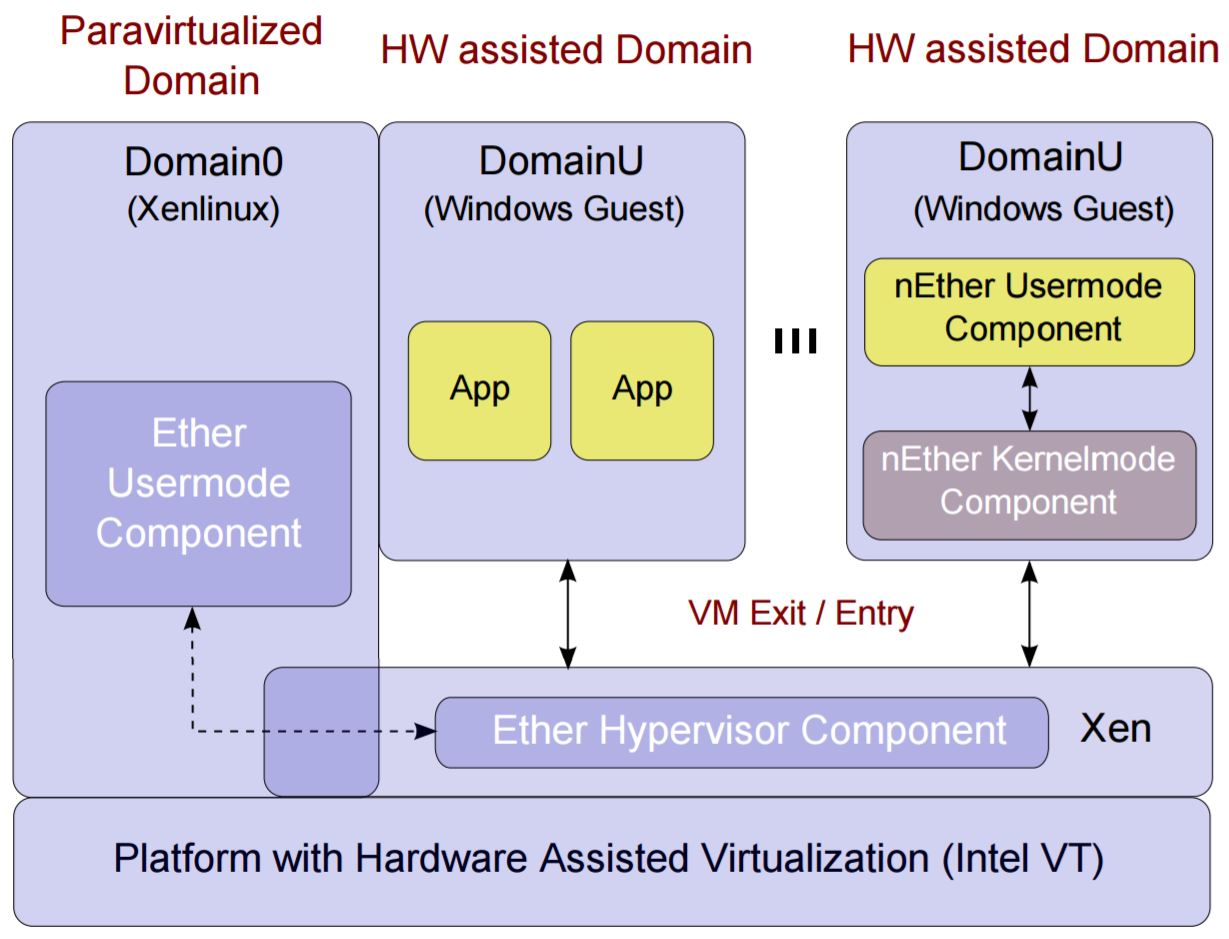
\includegraphics[width=\linewidth]{figure/nether.png}
	\caption{nEther's system overview.}
	\label{fig:nether}
\end{figure}

\subsection{Detecting Virtualized Environment}


\mvf{TODO: CPU Errata~\cite{thompson}}

Several efforts has been made on how relative difference in execution time of
two instructions could be used to detect a virtualized
environment~\cite{raffetseder2007, thompson}. Using absolute time differences is
not feasible, as architectures are complex and different, but the relative
difference is more predictable. Comparing one instruction that is known not to
be trapped by the VMM and one that is, for instance {\tt NOP} and {\tt CPUID}
the authors showed that different VMMs showed significantly different ratios
compared to bare metal.

Ferrie {et al.} showed in 2007 how~\cite{ferrie2007} context switches between an
VMM and guest could be used to detect hypervisors based on Intel VT-x though the
flushing of the Translation Lookaside Buffer (TLB). Using a non-privileged
instruction that is still trapped by the VMM, i.e. {\tt CPUID}, will cause a
flush of the TLB. This could be detected through timing the instruction before
and after anticipated flush. This method has later been documented by other
authors~\cite{thompson}.
\mvf{Maybe not relevant with use of ASID? (doesn't flush TLB)}

Using dynamic analysis to disable detection routines~\cite{kang2009}.

Using remote detector machine~\cite{franklin2008}.

%%% Local Variables:
%%% mode: latex
%%% TeX-master: "../paper"
%%% End:
